\section{Symmetries}
With the boundary conditions considered, the problem is symmetric about $b/2$. Therefor the problem may be redefined as the left half of the domain, with boundary $\Gamma=\Gamma_1\cup\Gamma_2\cup\Gamma_3\cup\Gamma_4$, see Figure~\ref{fig:domain_new}. \begin{Figure}
 \centering
 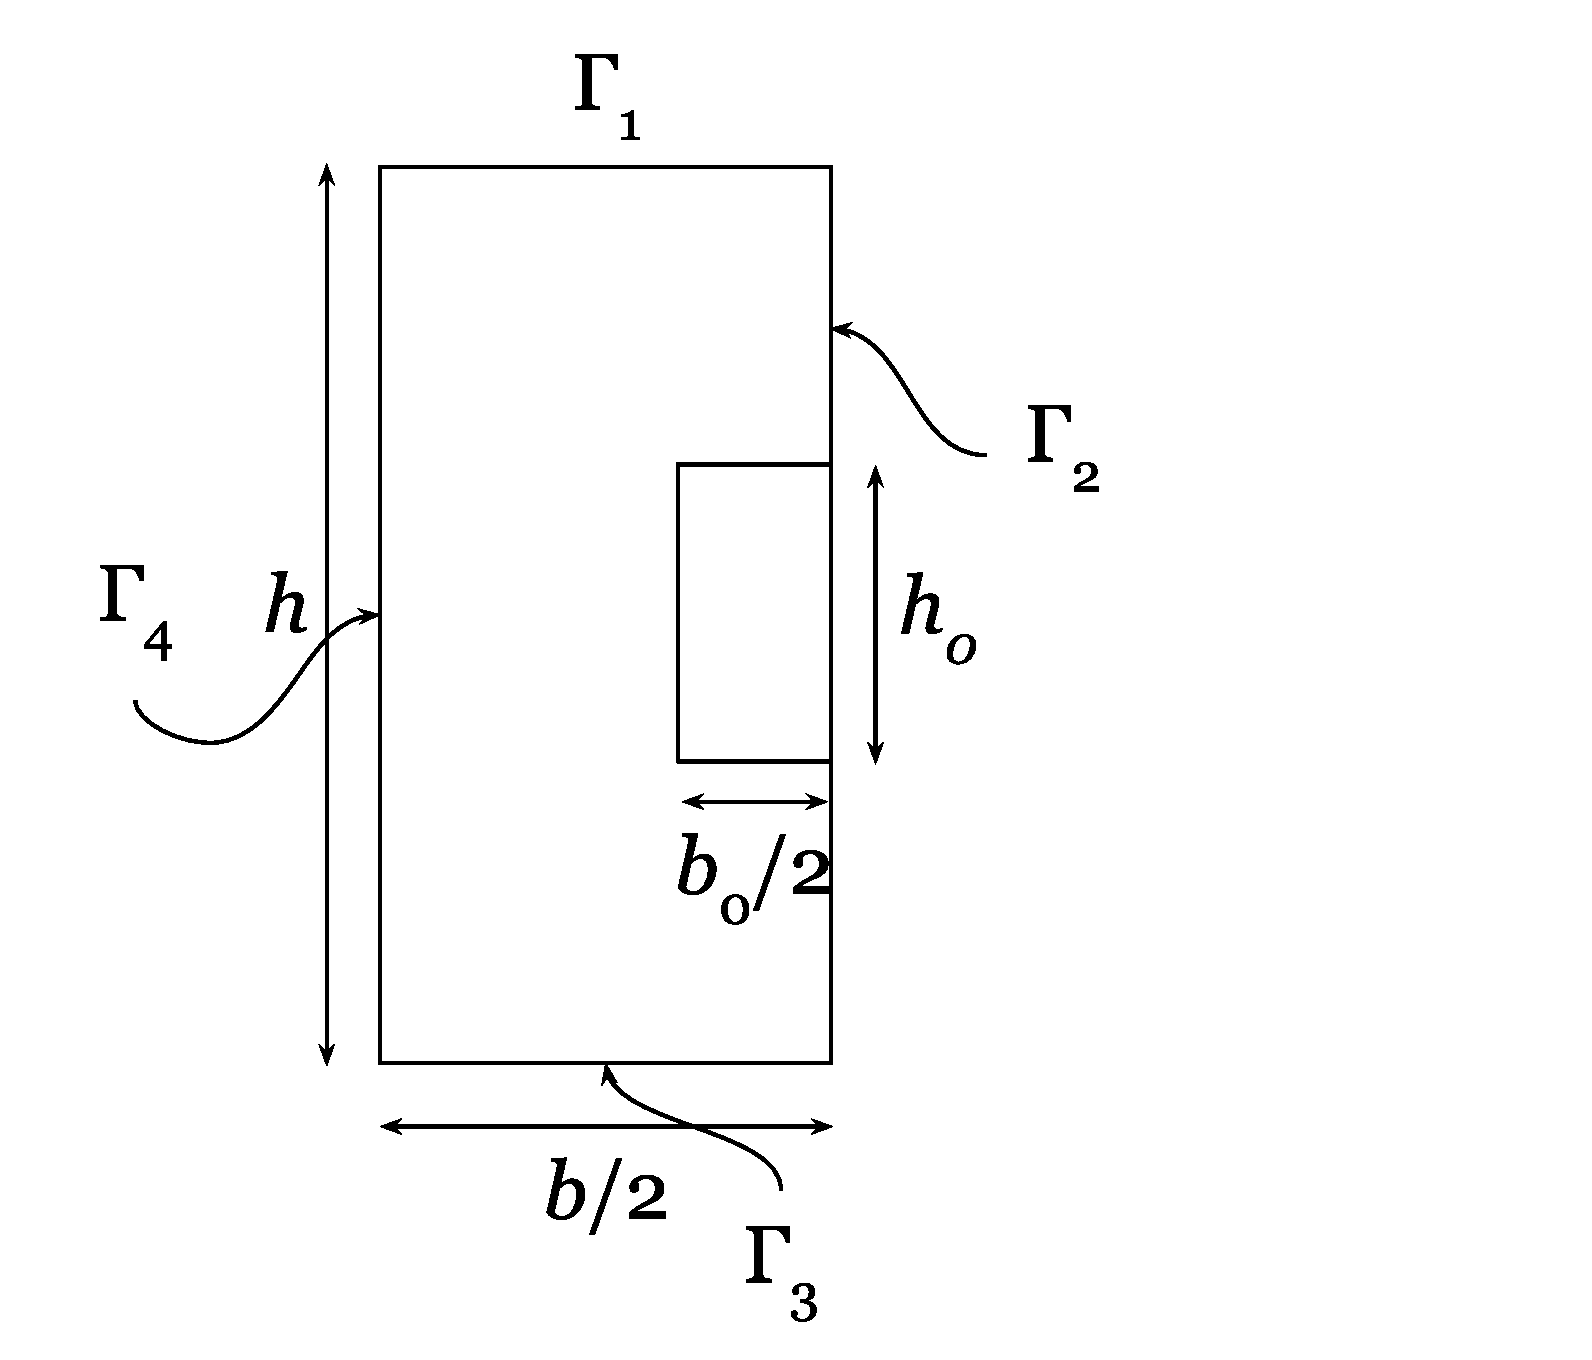
\includegraphics[width=0.7\linewidth]{domain_new.eps}
 \captionof{figure}{Newly defined domain $\Omega$.}\label{fig:domain_new}
\end{Figure} The boundary conditions become:
\begin{equation}
\begin{gathered}
    K\frac{\partial T}{\partial n}\arrowvert_{\Gamma_1\prime} = -\alpha \left(T_w - T_{\infty}\right),\\
    \frac{\partial T}{\partial n}\arrowvert_{\Gamma_2\prime} = 0,\\
    \frac{\partial T}{\partial n}\arrowvert_{\Gamma_3\prime} = 0,\\
    T\arrowvert_{\Gamma_4\prime} = T_0.
\end{gathered}\label{eq:bc}
\end{equation}.


\section{Minimization problem}
To derive the minimization problem for Eq. \ref{eq:heat}, theorem 5.8.1 from Numerical Methods in Scientific Computing \cite{kan}. To use this theorem, homogeneous boundary conditions are needed. Define $v=T-w$, where $w$ satisfies (\ref{eq:bc}). $v$ now satifies homogeneous boundary conditions. The operator in this problem is $L=-k\Delta$, and $L(T)=0$. $L$ needs to be self-adjoint, linear and positive over a space $\Sigma$. Where $\Sigma$ is a vector space consisting of all smooth functions satisfying the homogenous boundary conditions. $L$ is linear if $L(\alpha u+\beta v)=\alpha Lu+\beta Lv, \forall\alpha,\beta\in\mathbb{R}$:
\begin{gather*}
    L(\alpha u+\beta v)\\
    =-\Delta(\alpha u + \beta v)\\
    =-\alpha\Delta u-\beta \Delta v\\
    = \alpha Lu+\beta Lv.
\end{gather*}So L is linear.

$L$ is self-adjoint if $\int_\Omega uLv~\text{d}\Omega=\int_\Omega vLu~\text{d}\Omega, \forall u,v\in \Sigma$:
\begin{gather*}
    \int_\Omega uLv~\text{d}\Omega = -\int_\Omega u\Delta v~\text{d}\Omega\\
    =-\int_\Omega \nabla \cdot (u\nabla v) - \nabla u\cdot\nabla v~\text{d}\Omega
\end{gather*}
Using Gau\ss's theorem and the boundary conditions (\ref{eq:bc}):
\begin{gather*}
    =-\int_{\partial\Omega} u\frac{\partial v}{\partial n}~\text{d}\Gamma + \int_\Omega \nabla u\cdot\nabla v~\text{d}\Omega\\
    =\int_\Omega \nabla u\cdot \nabla v\text{d}\Omega
\end{gather*}
The same derivation also holds for $v$ and since $\int_\Omega \nabla u\cdot \nabla v~\text{d}\Omega = \int_\Omega \nabla v\cdot \nabla u~\text{d}\Omega$, $L$ is self-adjoint.

For $L$ to be positive aswell, $\int_\Omega uLu~\text{d}\Omega$ should be greater than or equation to 0, for all $u\in \Sigma$:
\begin{gather*}
    \int_\Omega uLu~\text{d}\Omega = - \int_\Omega u\Delta v~\text{d}\Omega\\
    = -\int_\Omega \nabla \cdot(u\nabla u) - \nabla u\cdot\nabla u~\text{d}\Omega
\end{gather*} Using Gau\ss's theorem and the boundary conditions (\ref{eq:bc}):
\begin{gather*}
    -\int_{\partial\Omega} u\frac{\partial u}{\partial n}~\text{d}\Gamma + \int_{\Omega} |\nabla u|^2~\text{d}\Omega \\
    =\int_\Omega |\nabla u|^2~\text{d}\Omega \geq 0.
\end{gather*} So $L$ is positive.

The minimization problem thus becomes:
\begin{equation}
    \min_{v\in\Sigma} F(v)=\frac{1}{2}\int_{\Omega}vLv~\text{d}\Omega + \int_{\Omega}vLw~\text{d}\Omega.
\end{equation} Since $w$ is unkown, it needs to be removed from the problem.

Subtitude $v=F-w$:
\begin{equation*}
F(T)=\frac{1}{2}\int_\Omega(T-w)(LT+Lw)~\text{d}\Omega.
\end{equation*} $w$ statisfies the boundary conditions, substituting them gives:
\begin{gather*}
    F(T) = \frac{1}{2}\int_{\Omega}(T-w)(-k\nabla (T+w))~\text{d}\Omega\\
    = \frac{1}{2}\int_{\Omega}\nabla\cdot\left[(T-w)\nabla(-k(T+w))\right]~\text{d}\Omega\\
    - \frac{1}{2}\int_{\Omega}\nabla(T-w)\cdot k\nabla(T+w)~\text{d}\Omega,
\end{gather*}using Gau\ss's theorem:
\begin{gather*}
    = -\frac{1}{2}\int_{\partial\Omega}(T-w)k\nabla(T+w)~\text{d}\Omega\\
    + \frac{1}{2}\int_{\Omega}\nabla(T-w)k\nabla(T+w)~\text{d}\Omega\\
    = -\frac{1}{2}\int_{\Omega}\nabla\cdot k\nabla T - \nabla W\cdot k\nabla w~\text{d}\Omega\\
    -\frac{1}{2}\int_{\partial\Omega}(T-w)k\nabla)(T+w)\text{d}\Gamma.
\end{gather*}Sinse the solution is independent of $w$, it can be left out in the first integral.
\begin{gather*}
    = \frac{1}{2}\int_{\Omega}\nabla T\cdot k\nabla T \text{d}\Omega \\
    -\frac{1}{2}\int_{\partial\Omega}(T-w)k\nabla (T+w)\text{d}\Gamma.
\end{gather*}

\section{Interface between the two materials} 
\section{Element matrices and vector}
Using Ritz' method: 
\begin{gather*}
    T(x,y) \simeq T_n(x,y)=\sum_{j=1}^n c_j\phi_j(x,y),\\
    \frac{\partial T_n}{\partial c_i}=\phi_i(x,y).
\end{gather*} Filling this in (\ref{eq:final}) gives:
\begin{gather*}
    \frac{\partial F}{\partial c_i} = \int_{\Omega}k\nabla T_n\cdot\nabla\phi_i~\text{d}\Omega\\
    +\int_{\Gamma_1}T_n\phi_i-\phi_iT_{\infty}~\text{d}\Gamma\\
    = \int_{\Omega}k\nabla(\sum_{j=1}^n)~\text{d}\Omega
\end{gather*}